% Stage 4: final project report. Covers everything (P0 to P6), verification, deviations,
% presentation feedback, how to run, and LLM disclosure. Compile from this folder:
% pdflatex stage4.tex (twice).
\documentclass[11pt,a4paper]{article}
\usepackage[margin=2.2cm]{geometry}
\usepackage[T1]{fontenc}
\usepackage{lmodern}
\usepackage{amsmath}
\usepackage{graphicx}
\usepackage{booktabs}
\usepackage{array}
\usepackage{enumitem}
\usepackage{xcolor}
\usepackage{caption}
\usepackage[hidelinks]{hyperref}
\graphicspath{{../experiments/}}
\setlist{itemsep=1pt,topsep=3pt}
\setlength{\parindent}{0pt}
\setlength{\parskip}{4pt}
\captionsetup{font=small,labelfont=bf}
\newcommand{\us}{\,$\mu$s}
\newcommand{\degC}{\,\textdegree C}
\newcommand{\todo}[1]{\textcolor{red}{[TODO: #1]}}
% Framed box standing in for an image that is still to be made: [width]{height}{what goes here}.
\newcommand{\imgplaceholder}[3][0.8]{\fbox{\parbox[c][#2][c]{#1\linewidth}{\centering\small
  \textcolor{gray}{[Image placeholder]}\\[2pt]\textcolor{gray}{#3}}}}

\begin{document}

\begin{center}
{\LARGE\bfseries Lightweight Temperature Predictor:\\[2pt] Calibrate Once, Predict Fast}\\[6pt]
{\large Final Project Report (Stage 4)}\\[4pt]
Ethan Bobby Kurien \quad Kaivalya Mase\\
Computer Architecture course project, topic: \emph{thermal management, lightweight temperature predictor}\\[2pt]
\today
\end{center}

\begin{abstract}
Dynamic thermal management (DTM) needs core temperatures every millisecond, and ideally a few
milliseconds ahead. The HotSpot simulator computes them accurately but needs 0.24\,s per steady
answer and 5.5\,ms per 1\,ms transient step. We built a two-stage predictor for heterogeneous
multicore floorplans. A one-time calibration runs HotSpot 8 times (steady) or 24 times (steady and
transient) per floorplan with 1\,W in one core at a time. The prediction stage then uses only the
stored coefficients. Because HotSpot without leakage is linear, the steady predictor (an influence
matrix) is exact to HotSpot's printed precision ($3\times10^{-5}$\,K worst) at 2.6\us\ per
prediction from under 1\,kB. The transient predictor (a sum of four exponentials per pair of
cores) is within 0.06--0.09\,K on average and 0.3\,K worst, at 3\us\ per step from about 4\,kB.
Every calibration-free alternative is 0.5--2.7\,K off on average. Used as a forecaster in a
closed loop with HotSpot, the predictor lets proactive DTM cut the time spent over the temperature
limit by 60--130$\times$ compared with reactive DTM, for 1--1.6\,\% throughput.
\end{abstract}

\tableofcontents
\newpage

%=====================================================================
\section{Introduction}
A modern chip has several cores. Under load they heat up, and above a limit they slow down, age
faster or fail. The chip's DTM software throttles cores (DVFS) to stay under the limit. To act
before the limit is crossed it needs fast predictions of temperature.

\textbf{Problem statement.} \emph{Develop a lightweight temperature predictor in two stages.
Calibration (one-time per floorplan): tune predictor coefficients for the given floorplan with
heterogeneous cores. Prediction: predict the temperature (steady state or transient) for a given
power input. Metrics: accuracy, prediction time, model size. Wishlist: show the effectiveness of
the predictor for proactive DTM.}

\textbf{Contributions.}
\begin{itemize}
  \item A trusted, fast HotSpot reference: a patched build with 6-decimal output, 29$\times$ faster
        transients (byte-identical) and a memory-leak fix.
  \item A calibration stage of 8 or 24 planned HotSpot runs per floorplan.
  \item An exact steady predictor (S1), a hot-spot predictor (S1-hot-max) and an accurate transient
        predictor and forecaster (T3), compared against baselines and an exact reduced model (T4).
  \item Evidence that per-floorplan calibration is needed (P1-3), and validation on 52 floorplans
        generated after the models were designed.
  \item Robustness studies: unusual inputs, package changes, leakage.
  \item A Python tool (\texttt{ltp}) for both stages.
  \item A closed-loop DTM demonstration with HotSpot as the chip.
\end{itemize}

%=====================================================================
\section{Background}
\textbf{HotSpot} \cite{hotspot} models the die and package (silicon, thermal interface, heat
spreader, heat sink) as a network of thermal resistances and capacitances. The grid model divides
the die into cells (here $64\times64$); the block model uses one node per block and is faster but
rougher \cite{hotspot4}.

\textbf{Linearity.} Without temperature-dependent leakage the network is linear, so rises scale
with power and add up across cores. Then $T = T_\text{amb} + G\,P$ in steady state, where
$G_{ij}$ is the rise of block $i$ per watt in core $j$.

\textbf{Related approaches.} Power blurring \cite{blurring} convolves the power map with a generic
kernel. ARX-type predictors \cite{coskun,singla} fit recent temperatures and powers. Compact
state-space models and their reductions \cite{matex,sharifi08,sharifi10} start from the thermal
network. Learned surrogates trained on many layouts report 0.35--1.3\,K error (IC-ThermBench). We
compare variants of all of these.

%=====================================================================
\section{Design approach}

\subsection{Two stages}
\begin{description}[leftmargin=1.2em]
  \item[Calibration] (once per floorplan): $N$ steady runs with 1\,W in core $j$ give column $j$ of
        $G$. $N$ short step runs (1\,ms sampling for 2\,s) and $N$ long step runs (20\,ms sampling
        for 100\,s) give the step response $s_{ij}(t)$ of every block to every core. For $N=8$ that
        is 24 runs.
  \item[Prediction] (many times): load the model file (about 8\,kB), give the power per core, get
        every block's temperature now (steady) or over time (transient).
\end{description}

\subsection{Models}
\begin{center}
\small
\begin{tabular}{@{}l p{7.6cm} l l@{}}
\toprule
Model & Idea & Calibration & Verdict \\
\midrule
S0 & Power blurring: generic kernel, no runs on the target \cite{blurring} & none & baseline \\
\textbf{S1} & Influence matrix: $T = T_\text{amb}+G P$ & 8 runs & \textbf{ship} \\
\textbf{S1-hot-max} & S1 for 3--9 candidate cells per core, take the max & same runs & \textbf{ship} \\
S2 / S2-lr & Compressed $G$: $k$ nearest cores + package term / low rank & from S1 & many cores only \\
T0 & Persistence: temperature stays as it is & none & baseline \\
T1 & First-order lag, one time constant per block & 24 runs & too simple \\
T2 & ARX fitted to one long trace \cite{coskun,singla} & 1 trace & 1-step forecasts \\
\textbf{T3} & Sum of $M$ exponentials, shared $\tau$, weights per pair & 24 runs & \textbf{ship} ($M=4$) \\
T4 & HotSpot's own network, reduced to $r$ states \cite{matex,sharifi08} & patched HotSpot & reference \\
\bottomrule
\end{tabular}
\end{center}

\textbf{S1.} $G[:,j] = T_\text{HotSpot}(\text{1\,W in core } j) - T_\text{amb}$. No fitting.

\textbf{S1-hot-max.} From the same runs' $64\times64$ maps, keep for each core the cells that were
its hottest point in any calibration run or at nominal power, and predict
$T_\text{hot}(c) = \max_{q} (T_\text{amb} + G^\text{cell}_{q\cdot} P)$.

\textbf{T3.} $s_{ij}(t) \approx \sum_m a_{ijm}(1-e^{-t/\tau_m})$ with $\sum_m a_{ijm} = G_{ij}$.
Fitted by variable projection: linear least squares for $a$ given $\tau$, nonlinear least squares
(SciPy trust-region) over $\log\tau$. At run time:
\begin{equation}
  z_{jm}[k+1] = \lambda_m z_{jm}[k] + (1-\lambda_m) P_j[k],\quad \lambda_m = e^{-\Delta t/\tau_m},
  \qquad T_i = T_\text{amb} + \sum_{j,m} a_{ijm} z_{jm}[k+1].
\end{equation}
For forecasting, T3 is \emph{anchored}: its forecast is shifted by the current difference between
sensor and model, $\hat T(k_0+h) = T_3(k_0+h) + (T_\text{sensor}(k_0) - T_3(k_0))$.

\textbf{T2 (ARX).} $x[k] = A_1 x[k-1] + A_2 x[k-2] + B_0 P[k] + B_1 P[k-1]$, fitted by ridge
regression on one recorded trace, with the steady gain constrained to equal $G$.

\textbf{T4.} A debug patch exports HotSpot's capacitances and conductances (16{,}396 nodes);
modal truncation to 200 modes, balanced truncation to $r$ states, and a first-order filter per
pair of cores for the dropped fast modes.

No model uses neural networks or other black-box learners. Ridge regression appears only in the
calibration-free baselines of P1-3.

\subsection{Evaluation}
\begin{itemize}
  \item Reference: HotSpot grid $64\times64$, the TA layer stack, HotSpot's example package,
        ambient 45\degC, $\Delta t = 1$\,ms.
  \item Test inputs are never used for calibration: TA nominal and maximum power and 300 random
        vectors per floorplan (steady); random phase traces of 2\,s and 10\,s (transient).
  \item Accuracy: mean and worst absolute error over cores; error in the peak; share of cases with
        the right hottest core. Time: median of 10{,}000 single calls, one thread. Size: stored
        coefficients $\times$ 8 bytes.
\end{itemize}

%=====================================================================
\section{Tools and implementation}
\begin{center}
\small
\begin{tabular}{@{}l p{11.3cm}@{}}
\toprule
Tool & Use \\
\midrule
HotSpot (grid model) & Ground truth for calibration and testing \\
Patched HotSpot & \texttt{setup/build\_hotspot\_ltp.sh} patches a copy: 6-decimal output; LU factorisation reused across transient steps (230\,ms $\to$ 5.5\,ms per step, byte-identical); a one-line memory-leak fix (a 60\,s trace needed 8\,GB, now flat at 115\,MB); output flushing for closed-loop use; a debug build that exports the network (T4) \\
Python 3, NumPy, SciPy & Predictor, fits, model reduction \\
Matplotlib & Figures \\
Ubuntu on WSL, Bash & Running HotSpot and experiments \\
Git and GitHub & Version control and collaboration \\
\bottomrule
\end{tabular}
\end{center}

\begin{center}
\small
\begin{tabular}{@{}l p{11.3cm}@{}}
\toprule
Path & Contents \\
\midrule
\texttt{src/sim/} & HotSpot runner and parser, floorplans, power generators, parallel runs and caching, closed-loop stepper, floorplan generators (\texttt{flpgen.py}, \texttt{tagen.py}) \\
\texttt{src/ltp/} & The predictor: models, calibration, \texttt{Predictor} class, command line, benchmark \\
\texttt{experiments/<ID>\_<name>/} & One folder per experiment: \texttt{run.py}, \texttt{README.md}, \texttt{results/} \\
\texttt{tests/test\_models.py} & Unit tests \\
\texttt{setup/}, \texttt{configs/} & HotSpot patches and build script; HotSpot configurations \\
\texttt{data/} & TA sample dataset, generated floorplans, generated traces \\
\bottomrule
\end{tabular}
\end{center}

%=====================================================================
\section{Data}
\begin{center}
\small
\begin{tabular}{@{}l p{8.5cm} c@{}}
\toprule
Set & Description & Floorplans \\
\midrule
TA 2D floorplans & 2 big (4$\times$4\,mm) + 6 little (2$\times$2\,mm) cores, FILL white space, 4 styles & 23 \\
HET-A & Our own heterogeneous layout with L2 and NoC blocks & 1 \\
HOM-16, HOM-64 & Synthetic grids of identical cores (compression tests) & 2 \\
EV6 & HotSpot's Alpha example with a real gcc power trace & 1 \\
Generated & \texttt{tagen.py}, 13 per TA style & 52 \\
\bottomrule
\end{tabular}
\end{center}
Power: nominal big 20\,W and little 8\,W (88\,W per chip); random vectors with big 10--20\,W and
little 5--10\,W; phase traces where every core switches between 4 levels with phases from 1\,ms to
2\,s. Three issues in the TA data were found: the Style\_2 power files put big-core power on little
cores (about 100\degC\ as given), s3\_fp004 is s3\_fp005 rotated, and the TA transient files are
constant. We therefore assign power by core size and generate our own traces.

%=====================================================================
\section{P0: a reference we can trust}
\begin{itemize}
  \item \textbf{Linearity (P0-2):} scaling, superposition and zero power all match to
        $10^{-6}$\,K, steady and transient.
  \item \textbf{Block vs grid (P0-3):} block model 1--5\,K off; $64\times64$ converged (0.15\,K
        from $128\times128$); hottest cell 3.3--4\,K above its core's average.
  \item \textbf{Infrastructure (P0-4):} 0.24\,s per steady run, 5.5\,ms per transient step, 8
        parallel runs is the sweet spot (memory-bound).
  \item \textbf{TA floorplans (P0-5):} 69--77\degC\ at nominal power; a little core is always the
        hottest (1.6$\times$ the power density).
\end{itemize}

\begin{figure}[h]
  \centering
  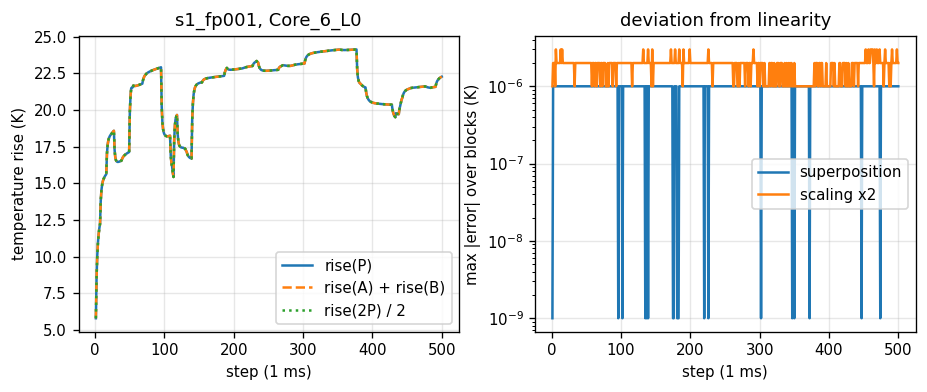
\includegraphics[width=0.48\linewidth]{P0-2_linearity/results/transient_linearity.png}\hfill
  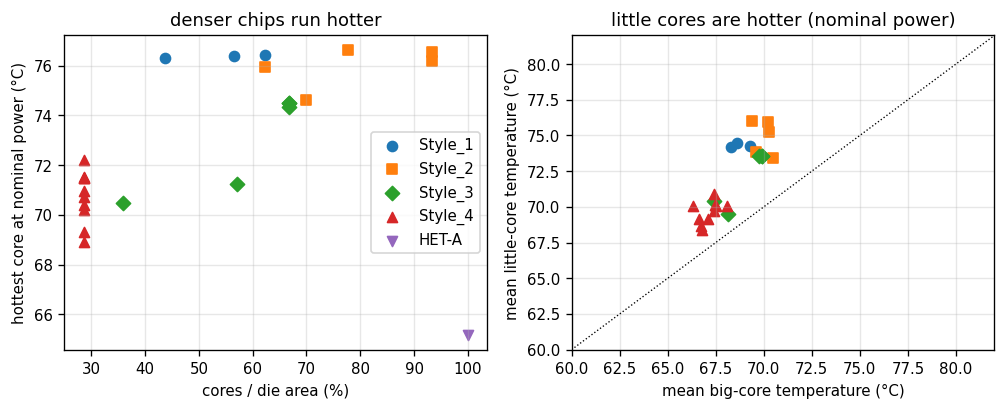
\includegraphics[width=0.48\linewidth]{P0-5_ta_floorplans/results/peak_vs_density.png}
  \caption{Left: one core's transient and its deviation from perfect linearity (about
  $10^{-6}$\,K). Right: denser floorplans run hotter; little cores are hotter than big ones.}
\end{figure}

%=====================================================================
\section{P1: calibration}

\subsection{P1-1: planned step runs}
24 runs per floorplan, 24 floorplans: 576 runs, 66\,min wall time. S1 needs only the 8 steady runs
(4.3\,s). The step responses have time constants of about 1\,ms, 3\,ms, 26\,ms, 89\,ms, 0.56\,s and
8.1\,s. A little core heats itself 2.4$\times$ as much per watt as a big core; edge cores up to
1.85\,K/W.

\begin{center}
\small
\begin{tabular}{@{}l c c c c c@{}}
\toprule
& T1 & T3 $M=2$ & $M=3$ & $M=4$ & $M=6$ \\
\midrule
Worst fit error (24 floorplans) & 14.1\,K & 2.82\,K & 1.04\,K & 0.46\,K & 0.12\,K \\
Size & 1.0\,kB & 1.9\,kB & 2.8\,kB & 3.7\,kB & 5.6\,kB \\
\bottomrule
\end{tabular}
\end{center}

\begin{figure}[h]
  \centering
  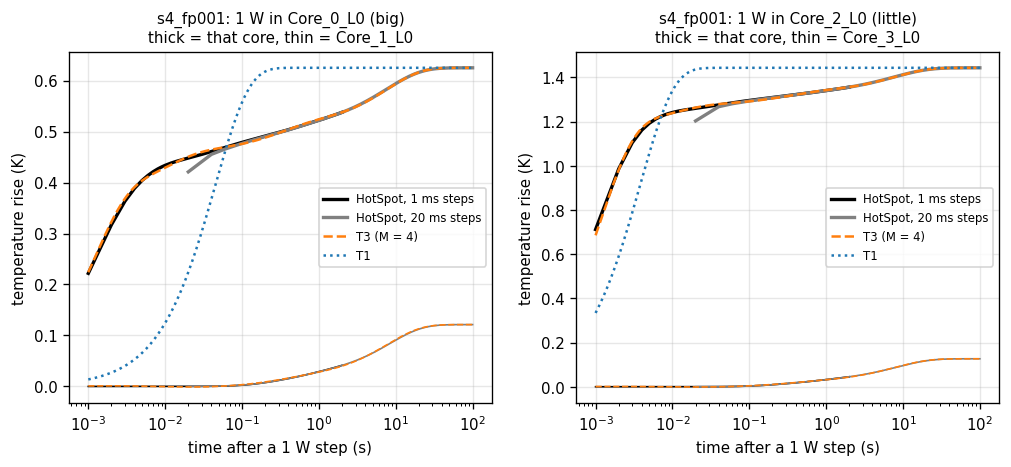
\includegraphics[width=0.9\linewidth]{P1-1_step_calibration/results/step_response_fits.png}
  \caption{Step responses to 1\,W in a big core (left) and a little core (right). HotSpot and T3
  overlap; T1 has the right final value but the wrong shape.}
\end{figure}

\subsection{P1-2: calibration from one trace (ARX)}
ARX needs a trace of at least about 5\,s; its best open-loop error is 0.21\,K mean and 1.0\,K worst
(20\,s trace), and it gets worse with longer traces because the fit minimises the one-step error,
not the open-loop error. Three lags on all blocks were unstable. T3 from planned steps is
3--5$\times$ better and stable by construction.

\subsection{P1-3: is calibration needed?}
\begin{center}
\small
\begin{tabular}{@{}l c c c c@{}}
\toprule
Method & Runs on target & Mean & Worst & Hottest core right \\
\midrule
S1, calibrated & 8 & 0.000007\,K & 0.00003\,K & 100\,\% \\
S0 + learned correction & 0 & 0.55\,K & 3.4\,K & 80\,\% \\
S0 power blurring & 0 & 0.76\,K & 5.2\,K & 71\,\% \\
Borrow a Style\_4 neighbour's $G$ & 0 & 1.11\,K & 5.2\,K & 60\,\% \\
One model per core type & 0 & 1.34\,K & 8.3\,K & 61\,\% \\
Geometry regression (+40 generated) & 0 & 1.94 (2.13)\,K & 7.4 (7.6)\,K & 42 (40)\,\% \\
Borrow s1\_fp001's $G$ everywhere & 0 & 2.66\,K & 12.1\,K & 45\,\% \\
\bottomrule
\end{tabular}
\end{center}
On 6{,}946 unseen runs, calibration wins by four orders of magnitude, even on Style\_4 where only
the core positions differ.

%=====================================================================
\section{P2: steady-state predictor}

\subsection{P2-1: S0, S1, S2}
\begin{center}
\small
\begin{tabular}{@{}l c c c c c@{}}
\toprule
Model (7{,}248 runs, 24 floorplans) & Mean & Worst & Time & Size & vs HotSpot \\
\midrule
S0 (uncalibrated) & 0.77\,K & 5.2\,K & 2.5\us & 928\,B & 94{,}000$\times$ \\
S1 & 0.000006\,K & 0.00003\,K & 2.6\us & 928\,B & 91{,}000$\times$ \\
S1, 32-bit & 0.000006\,K & 0.00003\,K & 3.1\us & 464\,B & 77{,}000$\times$ \\
S1, 302 inputs per call & same & same & 0.06\us\ each & 928\,B & 4{,}000{,}000$\times$ \\
S2, $k=2$ & 0.20\,K & 2.3\,K & 8.0\us & 507\,B & 30{,}000$\times$ \\
S2-lr, rank 2 & 3.1\,K & 12.1\,K & 3.4\us & 360\,B & 71{,}000$\times$ \\
\bottomrule
\end{tabular}
\end{center}
On HOM-64 (64 cores) S2 with 8 neighbours shrinks $G$ from 32.8\,kB to 5.7\,kB at 0.59\,K worst;
low rank fails (3.3\,K) because heat flow is local.

\subsection{P2-2: layout effects}
Edges (up to 27\,\% more self-heating), distance (coupling 0.63 $\to$ 0.15\,K/W over 4\,mm) and
die size (package term 0.10--0.14\,K/W) make each $G$ unique. Peak temperature rises with core
coverage ($r=+0.83$).

\subsection{P2-3 and P2-4: hot spots}
\begin{center}
\small
\begin{tabular}{@{}l c c c c@{}}
\toprule
Model (1{,}380 runs) & Size & Mean & Worst & Hottest core right \\
\midrule
Core average (plain S1) & 512\,B & 2.73\,K & 8.96\,K & 50\,\% \\
Average + fixed offset & 576\,B & 0.59\,K & 4.11\,K & 82\,\% \\
One fixed hottest cell & 512\,B & 0.29\,K & 3.97\,K & 68\,\% \\
S1-hot-max & 3.1\,kB & 0.078\,K & 1.6\,K & 90\,\% \\
All cells (exact) & 115\,kB & 0.000007\,K & 0.00003\,K & 100\,\% \\
\bottomrule
\end{tabular}
\end{center}
The hot spot moves in 61\,\% of cases, so fixed offsets fail. On HOM-64, S1-hot-max is 387\,kB
(194\,kB in 32-bit at no loss); S2-style compression gives 20--54\,kB at 0.15--0.33\,K mean.

\begin{figure}[h]
  \centering
  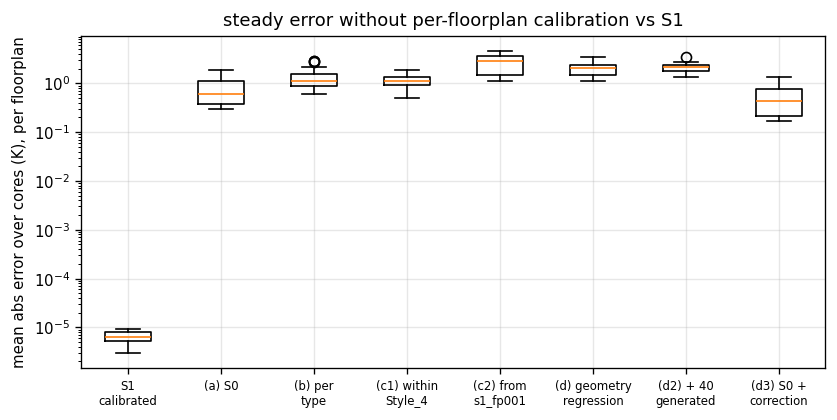
\includegraphics[width=0.48\linewidth]{P1-3_is_calibration_needed/results/error_by_method.png}\hfill
  \imgplaceholder[0.48]{4.5cm}{Error of each hot-spot predictor (P2-3).
  \texttt{hot\_spot\_error.png} does not exist; \texttt{size\_vs\_error.png} might replace it.}
  \caption{Left: error by method in P1-3. Right: error of each hot-spot predictor.}
\end{figure}

%=====================================================================
\section{P3: transient predictor}

\subsection{P3-1: open loop}
\begin{center}
\small
\begin{tabular}{@{}l c c c c@{}}
\toprule
Model (24 floorplans, 2\,s traces) & Mean & Worst & Time per step & Size \\
\midrule
T1 & 7.25\,K & 14.6\,K & 1.5\us & 1.0\,kB \\
T3, $M=2$ / 3 & 0.92 / 0.19\,K & 2.9 / 1.1\,K & 3.0\us & 1.9 / 2.8\,kB \\
T3, $M=4$ & 0.090\,K & 0.30\,K & 3.1\us & 3.7\,kB \\
T3, $M=6$ & 0.0093\,K & 0.13\,K & 3.2\us & 5.6\,kB \\
T2 ARX (main 4) & 0.19\,K & 0.57\,K & 5.4\us & 6.2\,kB \\
T3 $M=4$, EV6 + gcc & 0.073\,K & 0.21\,K & 4.4\us & 28.8\,kB \\
\bottomrule
\end{tabular}
\end{center}

\subsection{P3-2: forecasting}
\begin{center}
\small
\begin{tabular}{@{}l c c c c@{}}
\toprule
Model (mean error) & 1\,ms & 10\,ms & 100\,ms & 1\,s \\
\midrule
Persistence & 0.013\,K & 0.11\,K & 0.69\,K & 2.7\,K \\
T1 from sensors & 0.88\,K & 3.6\,K & 4.7\,K & 4.2\,K \\
T3 open loop & 0.06\,K & 0.06\,K & 0.06\,K & 0.06\,K \\
T3 anchored & 0.0009\,K & 0.0044\,K & 0.017\,K & 0.055\,K \\
T2 ARX from sensors & 0.0013\,K & 0.015\,K & 0.10\,K & 0.42\,K \\
\bottomrule
\end{tabular}
\end{center}
Persistence is up to 8\,K wrong 10\,ms ahead. Anchored T3 is best from 10\,ms to 1\,s.

\begin{figure}[h]
  \centering
  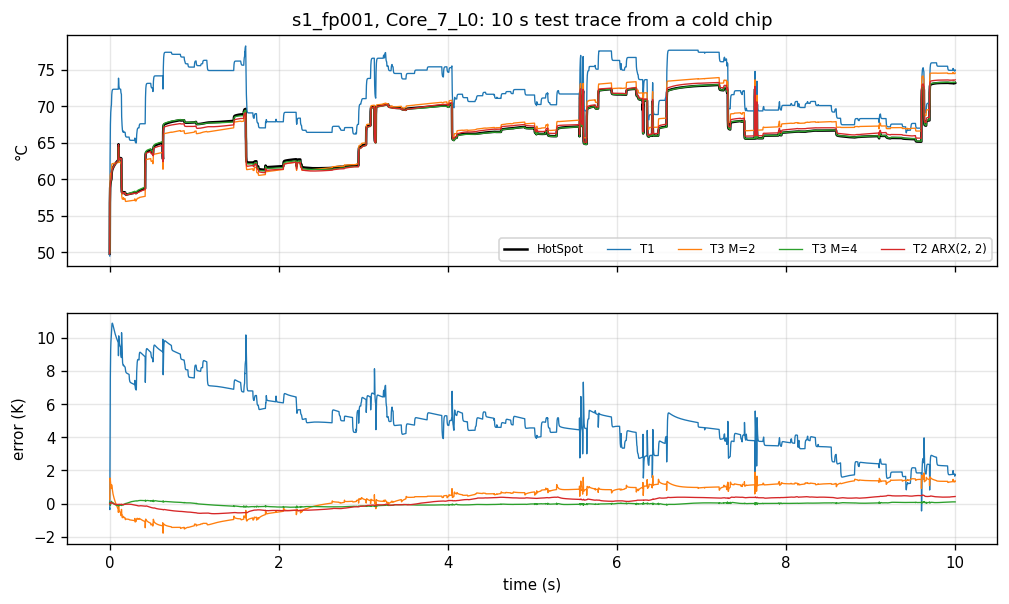
\includegraphics[width=0.48\linewidth]{P3-1_transient_predictor/results/trace_example.png}\hfill
  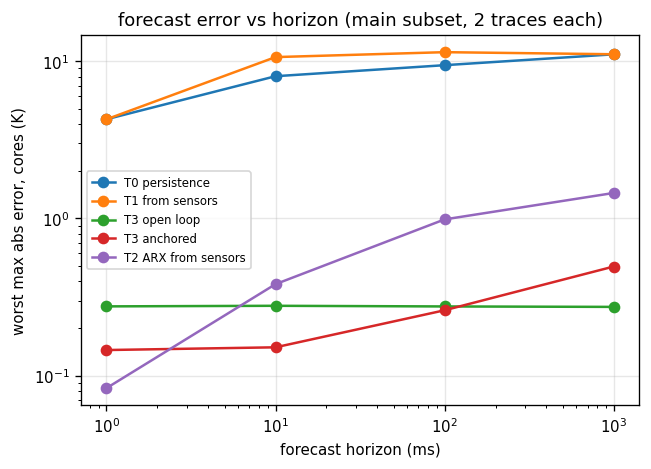
\includegraphics[width=0.48\linewidth]{P3-2_forecast_horizon/results/error_vs_horizon.png}
  \caption{Left: T3 on a test trace, on top of HotSpot. Right: forecast error against horizon.}
\end{figure}

\subsection{P3-3 and P3-4: trade-offs and the exact model}
T3 is the Pareto front from 2 to 6\,kB; T4 only wins below 0.05\,K (from about 16\,kB). HotSpot's
exported network reproduces HotSpot to $10^{-6}$\,K and its steady gain equals $G$. Reduced to 32
states it gives 0.047\,K worst; without the fast-mode filter the error stalls at 3.3\,K.

\begin{figure}[h]
  \centering
  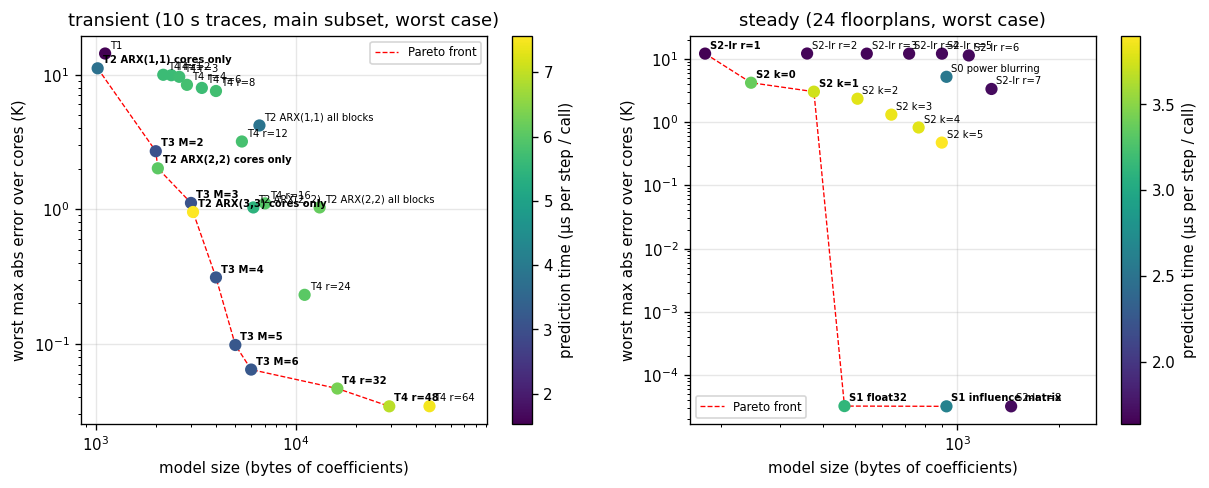
\includegraphics[width=0.48\linewidth]{P3-3_pareto/results/pareto.png}\hfill
  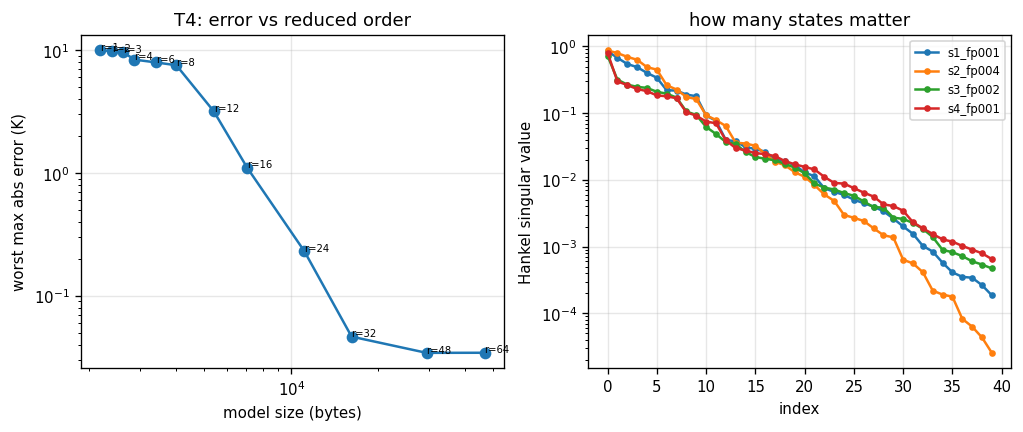
\includegraphics[width=0.48\linewidth]{P3-4_state_space_T4/results/t4_reduction.png}
  \caption{Left: size against worst error; Pareto front in bold. Right: T4 error against states.}
\end{figure}

%=====================================================================
\section{Extended validation: 52 generated floorplans}
\begin{center}
\small
\begin{tabular}{@{}l c c c c@{}}
\toprule
Set & S1 mean & S1 worst & T3 mean & T3 worst \\
\midrule
52 generated floorplans & $6.5\times10^{-6}$\,K & $3.4\times10^{-5}$\,K & 0.091\,K & 0.34\,K \\
24 TA floorplans & $6\times10^{-6}$\,K & $3\times10^{-5}$\,K & 0.090\,K & 0.30\,K \\
\bottomrule
\end{tabular}
\end{center}
The results carry over; per style, T3 ranges from 0.056\,K (Style\_4) to 0.114\,K (Style\_2). T3
picks the right hottest core in 88--100\,\% of steps and was slightly too cool at $t=2$\,s, so a
limit needs a margin of a few tenths of a kelvin.

\begin{figure}[h]
  \centering
  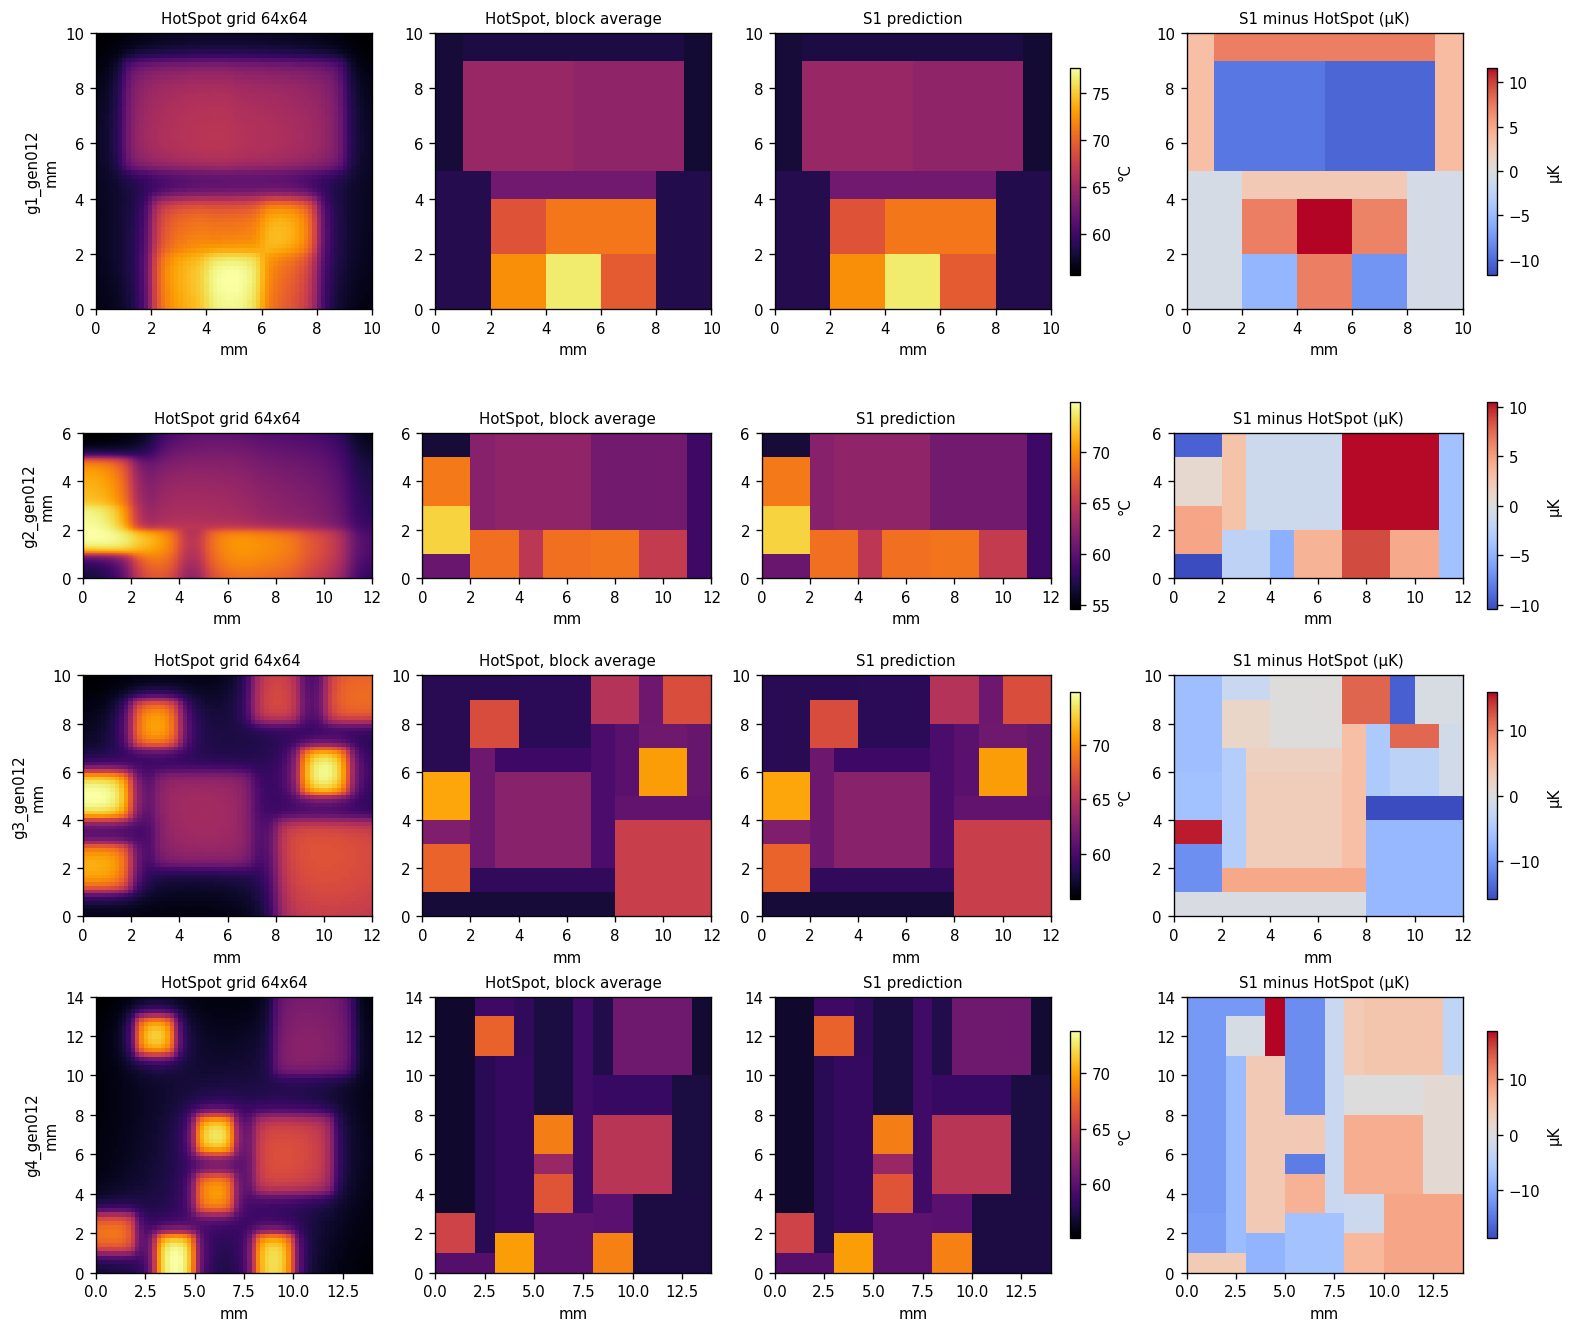
\includegraphics[width=0.9\linewidth]{extended_validation/results/heatmaps.png}
  \caption{One generated floorplan per style: HotSpot's $64\times64$ map, HotSpot's block
  averages, S1's prediction, and S1 minus HotSpot in micro-kelvin.}
\end{figure}

%=====================================================================
\section{P4: robustness}
\textbf{Unusual inputs (P4-1).} Power at 2--3$\times$ the maximum, bursty power (1--5\,ms
phases), task migration and warm starts are all fine (T3 worst 0.27--0.64\,K). The weak spot is a
different time step (0.1\,ms or 10\,ms: about 2\,K worst); calibrate at the controller's time step.

\textbf{Package change (P4-2).} New ambient: update $T_\text{amb}$ only (0.00002\,K). Heat-sink
resistance doubled or halved: the old model is 8.5\,K or 4.4\,K off; recalibrating (24 runs)
restores 0.00001--0.00002\,K.

\textbf{Leakage (P4-3).} Ignoring leakage costs 0.1\,K (default strength) or 1\,K (10$\times$). A
3--4 iteration fixed-point loop brings it to $6\times10^{-5}$\,K in 22--33\us. Steady state only,
since HotSpot does not support leakage in transients.

%=====================================================================
\section{P5: the \texttt{ltp} tool}
\texttt{ltp} (\emph{lightweight thermal predictor}) packages both stages of the predictor as one
command-line tool and one Python class. The calibration stage runs HotSpot and writes a single
model file per floorplan; every prediction command afterwards needs only that file and NumPy, so
it can run on a machine without HotSpot.

\begin{figure}[h]
  \centering
  \imgplaceholder[0.9]{4.5cm}{Workflow diagram: floorplan folder (.flp, .lcf) $\rightarrow$
  \texttt{ltp calibrate} (24 HotSpot runs) $\rightarrow$ \texttt{model.npz} $\rightarrow$
  \texttt{steady} / \texttt{transient} / \texttt{forecast} (NumPy only); \texttt{bench} compares
  the model file with fresh HotSpot runs.}
  \caption{How the \texttt{ltp} commands fit together.}
  \label{fig:ltp-flow}
\end{figure}

\subsection{Installation}
\todo{replace with the final install steps once packaging is done, e.g.
\texttt{pip install .} from the repository root, and the \texttt{ltp} entry point.} Until then the
tool runs from the repository root as \texttt{python3 -m src.ltp <command>}. Requirements: Python 3
and NumPy for prediction; SciPy (T3 fit) and the patched HotSpot inside WSL
(\texttt{setup/build\_hotspot\_ltp.sh}) for \texttt{calibrate} and \texttt{bench}.

\subsection{Commands}
\begin{center}
\small
\begin{tabular}{@{}l p{5.6cm} p{4.6cm} c@{}}
\toprule
Command & Input & Output & HotSpot? \\
\midrule
\texttt{calibrate} & floorplan (TA folder or name); \texttt{-o} model file; \texttt{--M} (default 4); \texttt{--refresh} & model file (\texttt{.npz}) & yes \\
\texttt{steady} & model; \texttt{--power} (one vector, W) or \texttt{--ptrace} (one vector per row) & steady temperature of every block (\degC) & no \\
\texttt{transient} & model; \texttt{--ptrace}; \texttt{--dt} (default 1\,ms); \texttt{--warm}; \texttt{-o} & temperature trace (\degC, or a \texttt{.ttrace} file) & no \\
\texttt{forecast} & model; \texttt{--history} (past powers); \texttt{--temps} (sensor readings now, \degC); \texttt{--next} (planned powers) & forecast for each planned step (\degC) & no \\
\texttt{bench} & model; floorplan; \texttt{--n} (300 vectors); \texttt{--steps} (2000) & size, error and time against fresh HotSpot runs & yes \\
\bottomrule
\end{tabular}
\end{center}

\textbf{\texttt{calibrate}} runs the $3N$ planned HotSpot runs (Section~3.1; 24 for 8 cores) in
parallel, caches them in \texttt{\textasciitilde/ltp\_runs/calib/}, fits S1 and T3, and adds one
hot-spot row per core (its hottest cell at nominal power). A second call reuses the cache.
{\small\begin{verbatim}
python3 -m src.ltp calibrate s4_fp001 -o model_s4_fp001.npz
\end{verbatim}}

\textbf{\texttt{steady}} evaluates S1, $T = T_\text{amb} + G\,P$, for one power vector or for every
row of a \texttt{.ptrace} file (the TA files are read directly; columns are matched by name).
{\small\begin{verbatim}
python3 -m src.ltp steady model_s4_fp001.npz --power 20,20,8,8,8,8,8,8
\end{verbatim}}

\textbf{\texttt{transient}} runs T3 over a power trace, from a cold chip or, with \texttt{--warm},
from the steady state of the first row. With \texttt{-o} it writes a HotSpot-style
\texttt{.ttrace} (kelvin, 6 decimals), so existing HotSpot scripts can read it.
{\small\begin{verbatim}
python3 -m src.ltp transient model_s4_fp001.npz --ptrace trace.ptrace -o out.ttrace
\end{verbatim}}

\textbf{\texttt{forecast}} replays the power history to get T3's state, then predicts the next
steps under the planned powers, anchored on the sensor readings (Section~3.2).
{\small\begin{verbatim}
python3 -m src.ltp forecast model_s4_fp001.npz --history past.ptrace \
                            --temps T_now.txt --next plan.ptrace
\end{verbatim}}

\textbf{\texttt{bench}} checks a model file against fresh HotSpot runs on unseen inputs and reports
the three metrics.
{\small\begin{verbatim}
python3 -m src.ltp bench model_s4_fp001.npz s4_fp001
\end{verbatim}}

\begin{figure}[h]
  \centering
  \imgplaceholder[0.46]{4cm}{Terminal screenshot: \texttt{ltp calibrate s4\_fp001} and
  \texttt{ltp steady} output}\hfill
  \imgplaceholder[0.46]{4cm}{Terminal screenshot: \texttt{ltp bench} output on s4\_fp001}
  \caption{\texttt{ltp} in use. \todo{insert screenshots.}}
  \label{fig:ltp-cli}
\end{figure}

\textbf{Example: \texttt{bench} on s4\_fp001} (300 new steady vectors, a 2\,s test trace):
\begin{center}
\small
\begin{tabular}{@{}l c c c@{}}
\toprule
& Mean error & Worst error & Time \\
\midrule
Steady (S1) & $5.2\times10^{-6}$\,K & $1.4\times10^{-5}$\,K & 2.6\us\ per call \\
Transient (T3, $M=4$) & 0.051\,K & 0.189\,K & 3.5\us\ per step \\
\bottomrule
\end{tabular}
\end{center}
The model file holds 8{,}032\,B of coefficients. \todo{re-run \texttt{bench} on the final code
and update these numbers.}

\begin{figure}[h]
  \centering
  \imgplaceholder[0.75]{5cm}{Plot: \texttt{ltp transient} output (\texttt{out.ttrace}) against
  HotSpot's \texttt{.ttrace} for the same \texttt{.ptrace}, hottest core of s4\_fp001}
  \caption{Output of \texttt{ltp transient} against HotSpot. \todo{generate.}}
  \label{fig:ltp-trace}
\end{figure}

\subsection{The model file}
One \texttt{.npz} file per floorplan (NumPy's archive format, readable from any language with an
\texttt{.npz} reader):
\begin{center}
\small
\begin{tabular}{@{}l l p{8cm}@{}}
\toprule
Entry & Shape & Meaning \\
\midrule
\texttt{names}, \texttt{power\_names} & $n$, $N$ & output blocks and power inputs, in order \\
\texttt{t\_amb} & scalar & ambient temperature (K) \\
\texttt{G} & $n \times N$ & S1 influence matrix (K/W) \\
\texttt{A}, \texttt{tau} & $n \times N \times M$, $M$ & T3 weights $a_{ijm}$ (K/W) and time constants (s) \\
\texttt{G\_hot}, \texttt{hot\_names} & $N \times N$, $N$ & optional: hot-spot rows, one per core \\
\bottomrule
\end{tabular}
\end{center}
For s4\_fp001 ($n = 25$ blocks, $N = 8$ cores, $M = 4$): $G$ is 1{,}600\,B and T3 6{,}432\,B, 8{,}032\,B
in total.

\subsection{Python interface}
The same model is available as a class, for use inside a simulator or a DTM controller:
\begin{center}
\small
\begin{tabular}{@{}l p{10cm}@{}}
\toprule
Method & Returns \\
\midrule
\texttt{Predictor.load(path)} & the predictor stored in a model file \\
\texttt{steady(P)} & steady temperatures (K) for one or many power vectors \\
\texttt{steady\_hot(P)} & hot-spot temperature of each core \\
\texttt{transient(P, dt, z0=None)} & temperature trace for a power trace \\
\texttt{step(z, p, dt)} & one time step: new state and temperatures (for online use) \\
\texttt{run\_state(P, dt)} & T3's state after a power history \\
\texttt{forecast(T\_now, z, P\_next, dt)} & anchored forecast for the planned powers \\
\texttt{size\_bytes()} & bytes of coefficients \\
\bottomrule
\end{tabular}
\end{center}
{\small\begin{verbatim}
from src.ltp.predictor import Predictor
p = Predictor.load("model_s4_fp001.npz")
T = p.steady([20, 20, 8, 8, 8, 8, 8, 8])            # every block, steady state
z = p.initial_state()                               # cold chip
for P_k in power_stream:                            # every 1 ms
    z, T_k = p.step(z, P_k, dt=1e-3)
T_next = p.forecast(T_sensors, z, P_plan, dt=1e-3)  # e.g. 20 ms ahead, for DTM
\end{verbatim}}
This is how the proactive controller of P6 uses the predictor.

\subsection{Testing}
\texttt{tests/test\_models.py} checks that S1 is exact on a linear system, that T3 recovers known
time constants and step responses, that ARX and T1 converge to $G$, and that a model file
round-trips through \texttt{save}/\texttt{load} and forecasts correctly. \todo{add the test run
output and any tests added for packaging.}

%=====================================================================
\section{P6: proactive DTM}

\subsection{P6-1: closed-loop HotSpot}
\texttt{src/sim/stepper.py} feeds HotSpot one power row at a time through a pipe and reads back
each temperature row (one patch flushes output after every row). It is identical (0\,K difference)
to a normal run, from a cold or warm chip.

\subsection{P6-2: reactive vs proactive DTM}
HotSpot acts as the chip for 4\,s runs. Each core requests power from a random workload; every
10\,ms the controller sets each core's speed (100\,\% down to 50\,\%). \emph{Reactive}: slow a
core that is over the limit. \emph{Proactive}: forecast 20\,ms ahead and choose the fastest speeds
whose forecast stays under the limit.

\begin{center}
\small
\begin{tabular}{@{}l l r r@{}}
\toprule
Floorplan (tight limit) & Policy & Core-ms over limit & Throughput \\
\midrule
s1\_fp001 (76.7\degC) & none & 10{,}400 & 1.000 \\
& reactive & 2{,}900 & 0.985 \\
& proactive, T3 & 22 & 0.975 \\
& proactive, T1 & 61 & 0.977 \\
& proactive, no model & 665 & 0.937 \\
\midrule
s4\_fp001 (68.6\degC) & none & 14{,}300 & 1.000 \\
& reactive & 3{,}890 & 0.976 \\
& proactive, T3 & 63 & 0.960 \\
& proactive, T1 & 100 & 0.963 \\
& proactive, no model & 1{,}500 & 0.908 \\
\bottomrule
\end{tabular}
\end{center}
Proactive DTM with T3 cuts the time over the limit 60--130$\times$ against reactive DTM, for
1--1.6\,\% throughput (0.1--0.2\,\% at the normal limit, where violations drop from 88--173 to
0--2 core-ms). Without a model, violations are 20--30$\times$ higher than with T3. Each decision
takes 0.4--0.7\,ms in Python (4--7\,\% of the interval).

\begin{figure}[h]
  \centering
  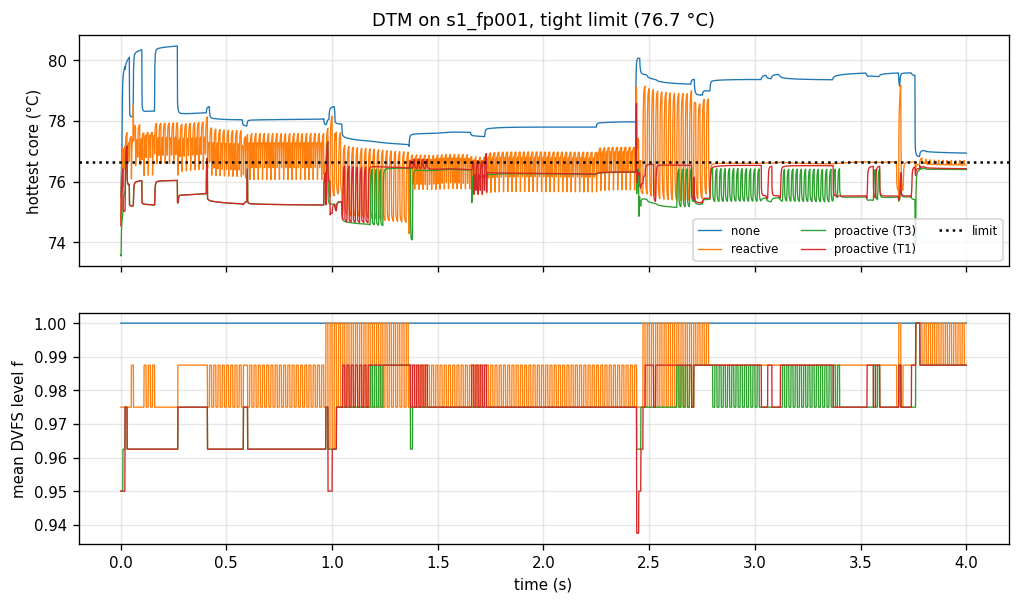
\includegraphics[width=0.75\linewidth]{P6-2_dtm/results/dtm_s1_fp001_tight.png}
  \caption{s1\_fp001, tight limit: reactive DTM saw-tooths around the limit; proactive stays just
  below it.}
\end{figure}

\subsection{P6-3: which cores should run the busy tasks?}
Scoring all 70 placements of 4 busy tasks on 8 cores, S1 picks the same coolest placement as
HotSpot on all 4 floorplans and ranks all 70 identically, in about 12\us\ against about 100
CPU-seconds (about 8{,}000{,}000$\times$ faster). The worst placement is 2.6--4.9\,K hotter than
the best, and the best placement differs per floorplan.

%=====================================================================
\section{Scorecard against our targets}
\begin{center}
\small
\begin{tabular}{@{}l l c c c@{}}
\toprule
& Metric & Target & Achieved & Status \\
\midrule
S1 & Mean error per block & $\le 0.1$\,K & 0.000006\,K & met \\
& Error in the peak & $\le 0.2$\,K & 0.00003\,K & met \\
& Hottest core right & $\ge 99\,\%$ & 100\,\% & met \\
& Time per prediction & $\le 20$\us & 2.6\us & met \\
& Model size & $\le 5$\,kB & 464--928\,B & met \\
& Calibration runs & $\le 9$ & 8 (4\,s) & met \\
\midrule
T3 & Mean error over a trace & $\le 0.5$\,K & 0.06--0.09\,K & met \\
& Error in the peak & $\le 1$\,K & 0.27--0.30\,K & met \\
& Hottest core right & $\ge 95\,\%$ & 96\,\% (worst floorplan) & met \\
& Time per step & $\le 50$\us & 3.1\us & met \\
& Model size & $\le 50$\,kB & 3.7--4\,kB & met \\
& Calibration time & $\le 2$\,min wall & $\approx 2.75$\,min & slightly over \\
\bottomrule
\end{tabular}
\end{center}
\todo{replace timings with the re-measurement on an idle machine, if done.}

%=====================================================================
\section{Verification approach}
\begin{enumerate}
  \item Verify the reference first: linearity, grid convergence, and a patched HotSpot whose output
        is byte-identical to the original.
  \item Separate calibration and test data strictly; learned baselines are trained
        leave-one-floorplan-out.
  \item Compare every model against HotSpot on all floorplans, and on 52 floorplans generated after
        the models were designed.
  \item Cross-check independently: HotSpot's own network (T4) gives the same $G$.
  \item Compare every model with a simpler baseline.
  \item Stress-test beyond nominal conditions (P4).
  \item Unit tests for the \texttt{ltp} package; closed-loop stepper checked against normal runs.
  \item Reproducibility: every HotSpot run is cached with its command, configuration and git
        commit; each experiment is one script with a README and results.
\end{enumerate}

%=====================================================================
\section{What went as planned, and what deviated}
All must-have deliverables and stretch goals were completed. Deviations:
\begin{center}
\small
\begin{tabular}{@{}p{3cm} p{4.3cm} p{7.7cm}@{}}
\toprule
Item & Planned & Done, and why \\
\midrule
HotSpot build & Precision patch & Also LU caching, memory-leak fix, flushing for closed loop: long traces were impractical or crashed. \\
Dataset & Our synthetic floorplans & TA's 23 as the main set, plus 52 generated in the same styles. \\
P1-3 & 4 baselines & Added generated-data and S0 + learned-correction variants. \\
S2 & One package term & One term per output block (global term up to 17\,K off). \\
P2-3 & One hottest cell & S1-hot-max: the hot spot moves. \\
T4 & Balanced truncation & Modal, then balanced truncation, then a fast-mode filter. \\
P6-1 & C stepper on HotSpot's library & HotSpot driven through pipes; simpler, identical. \\
P6-2 & DVFS and/or migration & DVFS only; migration left for future work. \\
Timing & One idle machine & One laptop, partly shared with HotSpot jobs. \\
\bottomrule
\end{tabular}
\end{center}

%=====================================================================
\section{Limitations and pending items}
\begin{itemize}
  \item All results are against HotSpot, not silicon measurements.
  \item Block-level models do not show hot spots inside a block, except through S1-hot-max.
  \item Leakage was tested in steady state only.
  \item A model is tied to its package: a new heat sink needs recalibration.
  \item \todo{\texttt{ltp} packaging for \texttt{pip install}: remove this item once done.}
  \item Open questions for the TA: the configuration used, the Style\_2 power files, and whether
        the FILL white space should leak.
\end{itemize}

%=====================================================================
\section{Learnings and future scope}
\textbf{Learnings.}
\begin{enumerate}
  \item HotSpot is linear without leakage, so a matrix predictor can be exact.
  \item Calibration is cheap (8 runs, 4\,s) and essential (0.5--2.7\,K without it).
  \item Position matters, not just core type.
  \item Little cores are the hot ones (2.4$\times$ self-heating per watt).
  \item Core averages hide hot spots 3--9\,K hotter, and the hot spot moves.
  \item Heat moves on time scales from 1\,ms to 8\,s: one time constant fails, four suffice.
  \item Planned step runs beat fitting a recorded trace.
  \item Forecasting needs a model: persistence is up to 8\,K wrong 10\,ms ahead.
  \item New ambient is free; a new heat sink needs recalibration.
  \item Proactive DTM with the predictor nearly eliminates overheating for about 1\,\% throughput.
\end{enumerate}

\textbf{Future scope.} Correcting a heat-sink change without new runs; leakage in transients;
multi-step ARX fitting; task migration between big and little cores as a DTM action; a vectorised
DTM controller (under 0.1\,ms per decision); calibration from real sensor data.

%=====================================================================
\section{Presentation feedback}
Feedback received during the presentation, and whether it was incorporated.
\begin{center}
\small
\begin{tabular}{@{}p{0.6cm} p{6.5cm} p{2.2cm} p{5.2cm}@{}}
\toprule
\# & Feedback & Incorporated? & Action taken / reason \\
\midrule
1 & \todo{feedback} & \todo{yes/no} & \todo{what was changed, or why not} \\
2 & & & \\
3 & & & \\
\bottomrule
\end{tabular}
\end{center}

%=====================================================================
\section{Submission contents and how to run}
\textbf{Archive contents.}
\begin{itemize}
  \item \texttt{reports/}: this report and the slides (PDF and \LaTeX\ source).
  \item \texttt{src/}: implementation (\texttt{sim/} HotSpot tooling, \texttt{ltp/} predictor).
  \item \texttt{experiments/}: one folder per experiment with \texttt{run.py}, README and results;
        \texttt{run.sh} runs any of them.
  \item \texttt{tests/}: unit tests.
  \item \texttt{setup/}, \texttt{configs/}: HotSpot patches, build script and configurations.
  \item \texttt{data/}: TA sample dataset and generated floorplans.
  \item \texttt{README\_SETUP.md}: setup and run instructions. \texttt{docs/guide.html}: a
        detailed guide to every experiment.
\end{itemize}

\textbf{How to run} (inside WSL, from the repository root):
{\small\begin{verbatim}
bash setup/build_hotspot_ltp.sh                 # one time: build the patched HotSpot
python3 tests/test_models.py                    # unit tests
bash experiments/run.sh P2-1_steady_predictor   # any experiment
python3 -m src.ltp calibrate s4_fp001 -o model.npz
python3 -m src.ltp steady model.npz --power 20,20,8,8,8,8,8,8
\end{verbatim}}
HotSpot runs are cached in \texttt{\textasciitilde/ltp\_runs/}. Run P1-1 first, then P1-2, then
the rest.

%=====================================================================
\section{LLM assistance disclosure}
We used Claude (Anthropic), through Claude Code, as an assistant. All output was reviewed and
checked by the team, and every number in this report comes from our own experiment outputs.
\begin{itemize}
  \item Drafting the project plan and the literature review.
  \item Drafting the floorplan generation script (\texttt{src/sim/flpgen.py}).
  \item Drafting this report and the presentation slides from the experiment READMEs.
  \item \todo{list every other use precisely, e.g. which code files, experiment scripts, figures
        or explanations were written or debugged with LLM help, and what was written by hand.}
\end{itemize}

%=====================================================================
\begin{thebibliography}{9}\small
\bibitem{hotspot} W.~Huang et al., ``HotSpot: A Compact Thermal Modeling Methodology for
  Early-Stage VLSI Design,'' \emph{IEEE TVLSI} 14(5):501--513, 2006.
\bibitem{hotspot4} W.~Huang et al., ``An Improved Block-Based Thermal Model in HotSpot 4.0 with
  Granularity Considerations,'' WDDD 2007.
\bibitem{matex} S.~Pagani, J.-J.~Chen, M.~Shafique, J.~Henkel, ``MatEx: Efficient Transient and
  Peak Temperature Computation for Compact Thermal Models,'' DATE 2015.
\bibitem{sharifi08} S.~Sharifi, C.~Liu, T.~S.~Rosing, ``Accurate Temperature Estimation for
  Efficient Thermal Management,'' ISQED 2008.
\bibitem{sharifi10} S.~Sharifi, T.~S.~Rosing, ``Accurate Direct and Indirect On-Chip Temperature
  Sensing for Efficient Dynamic Thermal Management,'' \emph{IEEE TCAD}, 2010.
\bibitem{blurring} A.~Ziabari et al., ``Power Blurring: Fast Static and Transient Thermal Analysis
  Method for Packaged Integrated Circuits and Power Devices,'' \emph{IEEE TVLSI} 22(11):2366--2379,
  2014.
\bibitem{coskun} A.~K.~Coskun, T.~S.~Rosing, K.~C.~Gross, ``Utilizing Predictors for Efficient
  Thermal Management in Multiprocessor SoCs,'' \emph{IEEE TCAD} 28(10), 2009.
\bibitem{singla} G.~Singla, G.~Kaur, A.~K.~Unver, U.~Y.~Ogras, ``Predictive Dynamic Thermal and
  Power Management for Heterogeneous Mobile Platforms,'' DATE 2015.
\end{thebibliography}

\end{document}
